\chapter{Theoretical foundations}
\label{chap:theoretical-foundations}

\section{Probability theory}
\label{sec:some-probability}

As we will see later, we will often be using probability distributions (in particular continuous probability distributions).

\subsection{Exponential distribution}
\label{sec:exponential-distribution}

The well-known exponential distribution is the central distribution we are dealing with in this text. All definitions and theorems within this subsection are along the lines of \cite{schickinger2001diskrete}.

\begin{definition}
  A continuous random variable is \emph{exponentially distributed} with parameter $\lambda$ if it has density 
  \begin{equation*}
    f(x) =
    \begin{cases}
      \lambda \cdot e^{-\lambda x} & \text{ if } x \geq 0 
      \\ 0 & \text{ otherwise}
    \end{cases}
    .
  \end{equation*}
\end{definition}

Note that the above definition also determines the distribution function $F$ of an exponentially distributed random variable as follows:

\begin{equation*}
  F(x) =
  \begin{cases}
    1-e^{\lambda x} & \text{ if } x \geq 0 \\
    0 & \text{ otherwise}
  \end{cases}
\end{equation*}

\begin{theorem}
  Let $X$ be an exponentially distributed random variable. Then, the expectancy of $X$ is $\E{X} = \frac 1 \lambda$.
\end{theorem}

\begin{proof}
  We can compute the expectancy for $X$ as follows:
  \begin{eqnarray*}
    \E{X} 
    &=& \int_{-\infty}^\infty x\cdot f(x)\, dx = \\
    &=& \int_{0}^\infty x\cdot \lambda e^{-\lambda x}\, dx \\
    &=& \left[ - \frac{e^{-\lambda x}\cdot \left( \lambda x + 1 \right)}{\lambda} \right]_{0}^\infty \\
    &=& \frac{1}{\lambda}
  \end{eqnarray*}
\end{proof}

\begin{theorem}[Scalability]
  Let $X$ be an exponentially distributed random variable with parameter $\lambda$ and let $a\in \mathbb{R}^+$. Then, the random variable $aX$ is exponentially distributed with parameter $\frac{\lambda}{a}$.
\end{theorem}

\begin{proof}
  We compute the probability that the random variable $aX$ is less than $x$:
  \begin{eqnarray*}
    \p{aX \leq x} 
    &=& \p{X \leq \frac{x}{a}} = \\
    &=& 1 - e^{-\frac{\lambda}{a} \cdot x}
  \end{eqnarray*}
  This result is equivalent to the density function of an exponentially distributed random variable with parameter $\frac{\lambda}{a}$.
\end{proof}

\begin{theorem}
  Let $X_1,\dots,X_n$ be exponentially-distributed random variables with respective parameters $\lambda_1,\dots,\lambda_n$. Then, the ranvom variable $Z:=\min_{i\in\left\{ 1,\dots,n \right\}} \left\{ X_i \right\}$ is exponentially distributed with parameter $\lambda=\lambda_1+\dots+\lambda_n$.
\end{theorem}

\begin{proof}
  We prove the claim by induction. 

  Suppose, we have two exponentially distributed random variables $X_1$ resp. $X_2$ with parameters $\lambda_1$ resp. $\lambda_2$. We then can compute
  \begin{align*}
    \p{min\left\{ X_1,X_2 \right\} \geq x} & = \p{X_1 \geq x \wedge X_2 \geq x} = \\ 
    & = \p{X_1 \geq x}\cdot\p{X_2 \geq x} = \\
    & = e^{-\lambda_1 x} \cdot e^{-\lambda_2 x} = \\
    & = e^{-\lambda_1 x - \lambda_2 x} = \\
    & = e^{-\left( \lambda_1+\lambda_2 \right) \cdot x},
  \end{align*}
  from which we can conclude that $\min\left\{ X_1,X_2 \right\}$ is exponentially distributed with parameter $\lambda_1 + \lambda_2$. By induction, we obtain our claim.
\end{proof}

\begin{definition}[Memorylessness]
  A random variable $X$ is called \emph{memoryless} if
  \begin{equation*}
    \p{X>t+s \mid X>s} = \p{X > t}
  \end{equation*}
\end{definition}

\begin{theorem}
  \label{sec:exponential-memoryless}
  Let $X$ be an exponentially distributed random variable with parameter $\lambda$. Then, $X$ is memoryless.
\end{theorem}

\begin{proof}
  We start by using the definition of conditional probability and rewrite until we arrive at our goal:
  \begin{eqnarray*}
    \p{X>t+s \mid X>s} &=& \frac{\p{X>t+s \wedge X>s}}{\p{X>s}} = \\
    &=& \frac{\p{X>t+s}}{\p{X>s}} = \\
    &=& \frac{e^{-\lambda \cdot(t+s)}}{e^{-\lambda s}} = \\
    &=& e^{-\lambda t} = \\
    &=& \p{X>t}
  \end{eqnarray*}
\end{proof}

This is a very advantageous property that can be exploited in our considerations to follow.

\emph{Remark:} It can even be shown that any memoryless continuous random variable is exponentially distributed, but theorem \ref{sec:exponential-memoryless} is sufficient for our needs.

\subsection{Uniform distribution}
\label{sec:uniform-distribution}

\begin{definition}
  A continuous random variable is \emph{uniformly distributed} over the interval $\left[ a,b \right]$ if it has density
  \begin{equation*}
    f(x) =
    \begin{cases}
      \frac{1}{b-a} & \text{ if } x\in\left[ a,b \right] \\
      0 & \text{ otherwise}
    \end{cases}.
  \end{equation*}
\end{definition}

The density of a uniform random variable is thus given by
\begin{equation*}
  F(x) = \begin{cases}
    0 & \text{ if } x<a \\
    \frac{x-a}{b-a} & \text{ if } x\in\left[ a,b \right] \\
    1 & \text{ if } x>b
  \end{cases}.
\end{equation*}


\subsection{General stuff}
\label{sec:probability-misc}

\begin{theorem}
  Let $X_1,\dots,X_n$ be independent, identically distributed, continuous random variables and let $i\in\left\{ 1,\dots,n \right\}$. Then 
  \begin{equation}
    \label{eq:probability-that-cont-random-variable-is-smallest-out-of-iid-is-one-over-n}
    \p{X_i = \min_{j\in\left\{ 1,\dots,n \right\}}\left\{ X_j \right\}} = \frac{1}{n}.
  \end{equation}
\end{theorem}

\begin{proof}
  It is clear that 
  \begin{equation*}
    \p{X_1 = \min_{j\in\left\{ 1,\dots,n \right\}}\left\{ X_j \right\}} = \p{X_2 = \min_{j\in\left\{ 1,\dots,n \right\}}\left\{ X_j \right\}} = \dots = \p{X_n = \min_{j\in\left\{ 1,\dots,n \right\}}\left\{ X_j \right\}},
  \end{equation*}
  because all random variables $X_1$ through $X_n$ behave the same. Thus we can deduce equation (\ref{eq:probability-that-cont-random-variable-is-smallest-out-of-iid-is-one-over-n}).
\end{proof}

\section{Graph theory}
\label{sec:foundations-graph-theory}

As we will see later, we will constantly deal with \emph{intrees}. In this section we develop simple notation for such trees. We assume that the reader is familiar with the concept of undirected trees and develop our notation on top of the one for undirected trees. For a more detailed introduction on what trees are, see e.g. \cite{diestel2005graph}.

\begin{definition}[Intree]
  Let $I'$ be a undirected tree. Let $v$ be a vertex within $I'$. Let $I$ be the directed version of $I'$ in such a way that all edges are directed towards vertex $v$. Then we call $I$ an intree or a rooted tree with root $v$.

  If there is an edge $(t_1, t_2)$ in $I$, we call $t_1$ a (direct) predecessor of $t_2$ and $t_2$ a (direct) successor of $t_1$. If there is a path from $t_1$ to $t_2$, we simply speak of predecessor and successor.
\end{definition}

Throughout this book, if not stated otherwise, we use the terms intree and tree interchangeably, because we are dealing only with intrees.

Those intrees can naturally be used to describe dependencies between different tasks, as long as each task is the requirement for at most one other tas. Each vertex in an intree then represents a task and if $t_1$ is a direct (direct) predecessor of $t_2$, this means that the task associated with $t_1$ must be executed before the task associated with $t_2$.

We can draw such intrees in a very straightforward manner: We draw the root at the bottom and its direct predecessors one level above. For each predecessor, we inductively repeat this procedure to obtain a ``top-to-bottom-description'' of the tree.

Figure \ref{fig:intree-example-task-names-directed-edges} shows an intree, where tasks 8 is a requirement for task 6, which itself is -- like task 7, 8 and (indirectly) task 10 -- a requirement for task 3. This figure also illustrates the fact that -- in an intree -- each task is a direct requirement for \emph{at most} one other task.

However, we are mostly interested in the \emph{structure} of the tree, which is why we most of the time omit the labellings of the vertices (i.e. we omit the task names) and rely on a \emph{unlabelled} representation as shown in figure \ref{fig:intree-example-structure-version}.

\begin{figure}[t]
  \centering
  \begin{subfigure}{.45\textwidth}
    \centering{}
    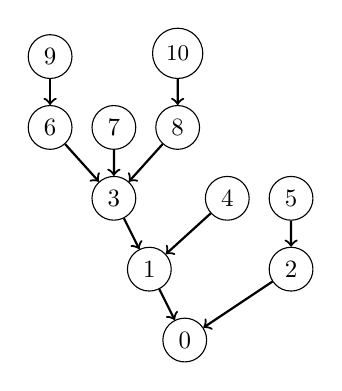
\begin{tikzpicture}[scale=.6, anchor=south]
      \node[circle, scale=0.9, draw] (tid0) at (3,1.5){0};
      \node[circle, scale=0.9, draw] (tid1) at (2.25,3){1};
      \node[circle, scale=0.9, draw] (tid2) at (1.5,4.5){3};
      \node[circle, scale=0.9, draw] (tid7) at (0.15,6){6};
      \node[circle, scale=0.9, draw] (tid9) at (0.15,7.5){9};
      \draw[<-, thick](tid7) -- (tid9);
      \node[circle, scale=0.9, draw] (tid10) at (1.5,6){7};
      \draw[<-, thick](tid2) -- (tid7);
      \draw[<-, thick](tid2) -- (tid10);
      \node[circle, scale=0.9, draw] (tid3) at (3.9,4.5){4};
      \node[circle, scale=0.9, draw] (tid5) at (2.85,6){8};
      \node[circle, scale=0.9, draw] (tid6) at (2.85,7.5){\small 10};
      \draw[<-, thick](tid5) -- (tid6);
      \draw[<-, thick](tid2) -- (tid5);
      \draw[<-, thick](tid1) -- (tid2);
      \draw[<-, thick](tid1) -- (tid3);
      \node[circle, scale=0.9, draw] (tid4) at (5.25,3){2};
      \node[circle, scale=0.9, draw] (tid8) at (5.25,4.5){5};
      \draw[<-, thick](tid4) -- (tid8);
      \draw[<-, thick](tid0) -- (tid1);
      \draw[<-, thick](tid0) -- (tid4);
    \end{tikzpicture}
    \caption{Labelled version with vertex labels and edges drawn as arrows.}
    \label{fig:intree-example-task-names-directed-edges}
  \end{subfigure}
  \quad
  \begin{subfigure}{.45\textwidth}
    \centering{}
    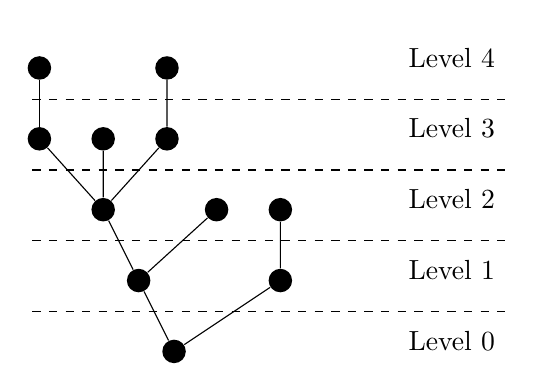
\begin{tikzpicture}[scale=.6, anchor=south]
      \node[circle, scale=0.9, fill] (tid0) at (3,1.5){};
      \node[circle, scale=0.9, fill] (tid1) at (2.25,3){};
      \node[circle, scale=0.9, fill] (tid2) at (1.5,4.5){};
      \node[circle, scale=0.9, fill] (tid7) at (0.15,6){};
      \node[circle, scale=0.9, fill] (tid9) at (0.15,7.5){};
      \draw[](tid7) -- (tid9);
      \node[circle, scale=0.9, fill] (tid10) at (1.5,6){};
      \draw[](tid2) -- (tid7);
      \draw[](tid2) -- (tid10);
      \node[circle, scale=0.9, fill] (tid3) at (3.9,4.5){};
      \node[circle, scale=0.9, fill] (tid5) at (2.85,6){};
      \node[circle, scale=0.9, fill] (tid6) at (2.85,7.5){};
      \draw[](tid5) -- (tid6);
      \draw[](tid2) -- (tid5);
      \draw[](tid1) -- (tid2);
      \draw[](tid1) -- (tid3);
      \node[circle, scale=0.9, fill] (tid4) at (5.25,3){};
      \node[circle, scale=0.9, fill] (tid8) at (5.25,4.5){};
      \draw[](tid4) -- (tid8);
      \draw[](tid0) -- (tid1);
      \draw[](tid0) -- (tid4);
      % level separators
      \draw[dashed] (0, 2.6) -- +(10, 0) node[below left, yshift=-.125cm]{Level 0};
      \draw[dashed] (0, 4.1) -- +(10, 0) node[below left, yshift=-.125cm]{Level 1};
      \draw[dashed] (0, 5.6) -- +(10, 0) node[below left, yshift=-.125cm]{Level 2};
      \draw[dashed] (0, 7.1) -- +(10, 0) node[below left, yshift=-.125cm]{Level 3};
      \draw[      ] (0, 8.6)    +(10, 0) node[below left, yshift=-.125cm]{Level 4};
    \end{tikzpicture}
    \caption{Unlabelled without arrows, edges are implicitly towards the root.}
    \label{fig:intree-example-structure-version}
  \end{subfigure}
  \caption{Graphical representation of an intree with 5 levels (numbered 0 to 4). All edges are implicitly directed towards the root, which is drawn at the bottom of the tree. Most of the time, the \emph{structure} of the tree is enough, so we will omit vertex names most of the time.}
  \label{fig:intrees-introductory-explanation}
\end{figure}

\begin{definition}[Level]
  Let $I$ be an intree. Let $v$ be a vertex within $I$. We define $level(v)$ be number of edges along the (unique) path from $v$ to the root.
\end{definition}

The concept of levels is illustrated in figure \ref{fig:intrees-introductory-explanation}.

\todo{Anzahl der rooted trees angeben.}

%%% Local Variables:
%%% TeX-master: "../thesis.tex"
%%% End: 